        %%******************************************%%
        %%                                          %%
        %%        Modello di tesi di laurea         %%
        %%            di Andrea Giraldin            %%
        %%                                          %%
        %%             2 novembre 2012              %%
        %%                                          %%
        %%******************************************%%

\begin{document}
    \frontmatter
    \begin{titlepage}
    \begin{center}
        \begin{LARGE}
            \textbf{\myUni}\\
        \end{LARGE}

        \vspace{10pt}

        \begin{Large}
            \textsc{\myDepartment}\\
        \end{Large}

        \vspace{10pt}

        \begin{large}
            \textsc{\myFaculty}\\
        \end{large}

        \vspace{30pt}
        \begin{figure}[htbp]
            \centering
            
\includegraphics[height=6cm]{unipd-logo}
        \end{figure}
        \vspace{30pt}

        \begin{LARGE}
            \textbf{\myTitle}\\
        \end{LARGE}

        \vspace{10pt}

        \begin{large}
            \textsl{\myDegree}\\
        \end{large}

        \vspace{40pt}

        \begin{large}
            \begin{flushleft}
                \textit{Relatore}\\
                \vspace{5pt}
                \profTitle\ \myProf
            \end{flushleft}

            % You can tweak the spacing to have professor and student names on the same line
            % useful if the page is broken by a long thesis title and you need more space
            \vspace{-52pt}

            \begin{flushright}
                \textit{Laureando}\\
                \vspace{5pt}
                \myName \\
                \vspace{5pt}
                \textit{Matricola} \myID
            \end{flushright}
        \end{large}

        \vspace{40pt}

        \line(1, 0){338} \\
        \begin{normalsize}
            \textsc{Anno Accademico \myAA}
        \end{normalsize}
    \end{center}
\end{titlepage}

    \clearpage
\phantomsection
\thispagestyle{empty}

\hfill
\vfill

\noindent\myName: \textit{\myTitle,}
\myDegree,
\textcopyright\ \myTime.

    \cleardoublepage
\phantomsection
\thispagestyle{empty}
\pdfbookmark{Dedica}{Dedica}

\vspace*{3cm}

\begin{center}
    Lorem ipsum dolor sit amet, consectetuer adipiscing elit. \\ \medskip
    --- Oscar Wilde
\end{center}

\medskip

\begin{center}
    Dedicato a ...
\end{center}

    \cleardoublepage
\phantomsection
\pdfbookmark{Sommario}{Sommario}
\begingroup
\let\clearpage\relax
\let\cleardoublepage\relax
\let\cleardoublepage\relax

\chapter*{Sommario}

Il presente documento descrive il lavoro svolto durante il periodo di stage dal laureando
Valerio Occhinegro presso l’azienda Spazio Dev Srl di Tombolo (PD). Lo stage, svoltosi al termine del percorso di studi della Laurea Triennale in "Scienze Informatiche", ha avuto una durata complessiva di 306 ore.

Il lavoro in questione è stato suddiviso in 4 diverse fasi, ognuna delle quali caratterizzata da obiettivi specifici e scadenze precise, e si basa su un'analisi intelligente di siti web, improntata alla vendita dei servizi aziendali a potenziali clienti. Il ruolo del laureando è quello di gestire e archiviare i siti web target e successivamente classificarli per fornire a Spazio Dev input utili per acquisire l'abilità di ampliare la quantità dei propri clienti in maniera rapida e automatizzata. 
Nello specifico, il progetto di stage ha l’obiettivo di sviluppare competenze avanzate nell’intelligenza artificiale, con un focus
particolare sulla classificazione e organizzazione dei dati; uno studio che si inserisce nel contesto di
{“SalesCRM: Customer Relationship Manager ”, un sistema integrato che mira a ottimizzare la gestione delle relazioni con i clienti e a migliorare l’efficienza dei venditori.} INSERIRE VERO TITOLO
Lo scopo ultimo del progetto è la creazione di un sistema intelligente che sia in grado di analizzare dataset complessi,
classificare la qualità dei siti web (siti che potrebbero essere migliorati e siti che non necessitano di modifiche) e proporre i propri servizi alle aziende che ne necessitano in maniera automatica. 
Il laureando è responsabile dello sviluppo di funzionalità chiave del sistema che consentiranno di fornire
soluzioni strategiche agli utilizzatori della piattaforma. 



%\vfill

%\selectlanguage{english}
%\pdfbookmark{Abstract}{Abstract}
%\chapter*{Abstract}

%\selectlanguage{italian}

\endgroup

\vfill

    \cleardoublepage
\phantomsection
\pdfbookmark{Ringraziamenti}{ringraziamenti}

\begin{flushright}{
    \slshape
    ``Non importa quanto piano vai, finché non ti fermi''} \\
    \medskip
    --- Confucio
\end{flushright}


\bigskip

\begingroup
\let\clearpage\relax
\let\cleardoublepage\relax
\let\cleardoublepage\relax

\chapter*{Ringraziamenti}

\noindent \textit{
    Prima di tutto vorrei ringraziare profondamente il Prof. \myProf, per avermi aiutato durante la stesura di questa tesi; senza i suoi consigli e la sua disponibilità fuori dal comune avrei sicuramente scritto un elaborato di qualità inferiore. Ha svolto un lavoro talmente impeccabile da meritarsi tutta la mia stima e per quel poco che conta un po'di pubblicità positiva con i miei colleghi che devono ancora laurearsi.
    }\\

\noindent \textit{
    Ringrazio tutta la mia famiglia, i miei zii e i miei cugini per essermi stati vicini e avermi sostenuto in questi anni difficili.
    }\\

\noindent \textit{
    Dedico degli ulteriori ringraziamenti ai miei amici Irene, Paño, Alessia e Mattia che mi hanno aiutato a tenere alto il morale durante questo percorso; a tutti i colleghi universitari il cui supporto è stato di fondamentale importanza per superare gli ultimi esami e all'intero Dipartimento di Chimica per avermi ospitato innumerevoli volte.  
    }\\

\noindent \textit{
    Un ringraziamento particolare è riservato a Matteo che posso considerare un vero e proprio fratello maggiore (senza nulla da togliere a Claudia), lo ringrazio per avermi aiutato durante uno degli anni più faticosi e per avermi fatto appassionare al mondo della "Geomatica".
    }\\
\bigskip

\noindent\textit{\myLocation, \myTime}
\hfill \myName

\endgroup

    \cleardoublepage
\pdfbookmark{\contentsname}{tableofcontents}
\setcounter{tocdepth}{2}
\tableofcontents
%\markboth{\contentsname}{\contentsname}
\clearpage

\begingroup
    \let\clearpage\relax
    \let\cleardoublepage\relax
    \let\cleardoublepage\relax

    % Figures list
    \phantomsection
    \pdfbookmark{\listfigurename}{lof}
    \listoffigures

    \vspace*{8ex}

    \newpage
    % Tables list
    \phantomsection
    \pdfbookmark{\listtablename}{lot}
    \listoftables

    \vspace*{8ex}
\endgroup

\cleardoublepage

    \cleardoublepage

    \mainmatter
    \chapter{Introduzione}
\label{cap:introduzione}

Introduzione al contesto applicativo.\\

\noindent Esempio di utilizzo di un termine nel glossario \\
\gls{api}. \\

\noindent Esempio di citazione in linea \\
\cite{site:agile-manifesto}. \\

\noindent Esempio di citazione nel pie' di pagina \\
citazione\footcite{womak:lean-thinking} \\

\section{L'azienda}

Descrizione dell'azienda.

\section{L'idea}

Introduzione all'idea dello stage.

\section{Organizzazione del testo}

\begin{description}
    \item[{\hyperref[cap:processi-metodologie]{Il secondo capitolo}}] descrive ...
    
    \item[{\hyperref[cap:descrizione-stage]{Il terzo capitolo}}] approfondisce ...
    
    \item[{\hyperref[cap:analisi-requisiti]{Il quarto capitolo}}] approfondisce ...
    
    \item[{\hyperref[cap:progettazione-codifica]{Il quinto capitolo}}] approfondisce ...
    
    \item[{\hyperref[cap:verifica-validazione]{Il sesto capitolo}}] approfondisce ...
    
    \item[{\hyperref[cap:conclusioni]{Nel settimo capitolo}}] descrive ...
\end{description}

Riguardo la stesura del testo, relativamente al documento sono state adottate le seguenti convenzioni tipografiche:
\begin{itemize}
	\item gli acronimi, le abbreviazioni e i termini ambigui o di uso non comune menzionati vengono definiti nel glossario, situato alla fine del presente documento;
	\item per la prima occorrenza dei termini riportati nel glossario viene utilizzata la seguente nomenclatura: \emph{parola}\glsfirstoccur;
	\item i termini in lingua straniera o facenti parti del gergo tecnico sono evidenziati con il carattere \emph{corsivo}.
\end{itemize}

    \chapter{Processi e metodologie}
\label{cap:processi-metodologie}

In questo capitolo sono riassunti i processi e le metodologie che lo studente ha applicato durante lo sviluppo del progetto di stage. 

\section{Gestione della configurazione}
La gestione della configurazione è il processo tramite il quale è possibile identificare, controllare e coordinare i vari componenti del software e le risorse ad esso associate durante l'intero ciclo di vita del prodotto. Grazie a questo processo gli sviluppatori possono tenere traccia delle modifiche e gestire le varie versioni garantendo il funzionamento del prodotto nel tempo.

\subsection{Tecnologie di supporto}
Le tencologie utilizzate per il versionamento del prodotto sono:
\begin{itemize}
    \item Git: è un DVCS(Distributed Version Controll System) ampiamente diffuso che consente di gestire e monitorare i cambiamenti del codice e della documentazione. Questo strumento è fondamentale per avere una storia completa dello sviluppo da poter sfruttare in caso di necessità. Il codice viene inserito all'interno di un repository, ossia una cartella che contiene tutti i file relativi al progetto, dove è possibile salvare ogni cambiamento tramite commit. Il commit segnala ogni modifica e la data in cui viene attuata, è dunque sufficiente spostarsi tra i vari commit per tornare ad una versione più o meno aggiornata.    
    \item Gitea: è un servizio che supporta le repository di Git, è simile a GitHub, Bitbucket e GitLab, ma ha il vantaggio di essere self-hosted. 
    Tutti i repository aziendali sono mantenuti sul server interno, ciò consente di avere una risposta molto rapida.

    %commit e branch tutti i salcazzi vari
\end{itemize}

\section{Processo sviluppo prodotto}

%processo di sviluppo ci schiaffo lo scrum

%processi di supporto tutte le menate di documentazione ecc

%processi organizzativi, its, repo, formazione
    \chapter{Il progetto}
\label{cap:descrizione-stage}

\intro{Questo capitolo contiene le informazioni preliminari che sono state fornite allo studente e le misure preventivie adottate per iniziare la produzione.}\\

\section{Analisi del progetto}

Il progetto si basa sull'integrazione di un nuovo workflow all'interno di un applicativo preesistente; lo studente deve occuparsi dello sviluppo di una soluzione in grado di migliorare la portata dell'azienda per quanto riguarda il raggiungimento di nuovi clienti.

\subsection{SalesCRM}
SalesCRM è il CRM che viene utilizzato dai commerciali interni all'azienda; contiene tutte le informazioni relative ai contatti che sono stati raggiunti dal reparto vendite. 
Gli utenti sono in grado di immagazzinare i dati raccolti su clienti e potenziali clienti tramite un interfaccia intuitiva sviluppata utilizzando \nameref{tec:Laravel} e \nameref{tec:Filament}.

\subsubsection{Componenti principali}
\begin{itemize}
    \item Home page (Fig.~\ref{fig:salesCRM-home}) contenente grafici informativi.
    
    \begin{figure}[!h] 
        \centering 
        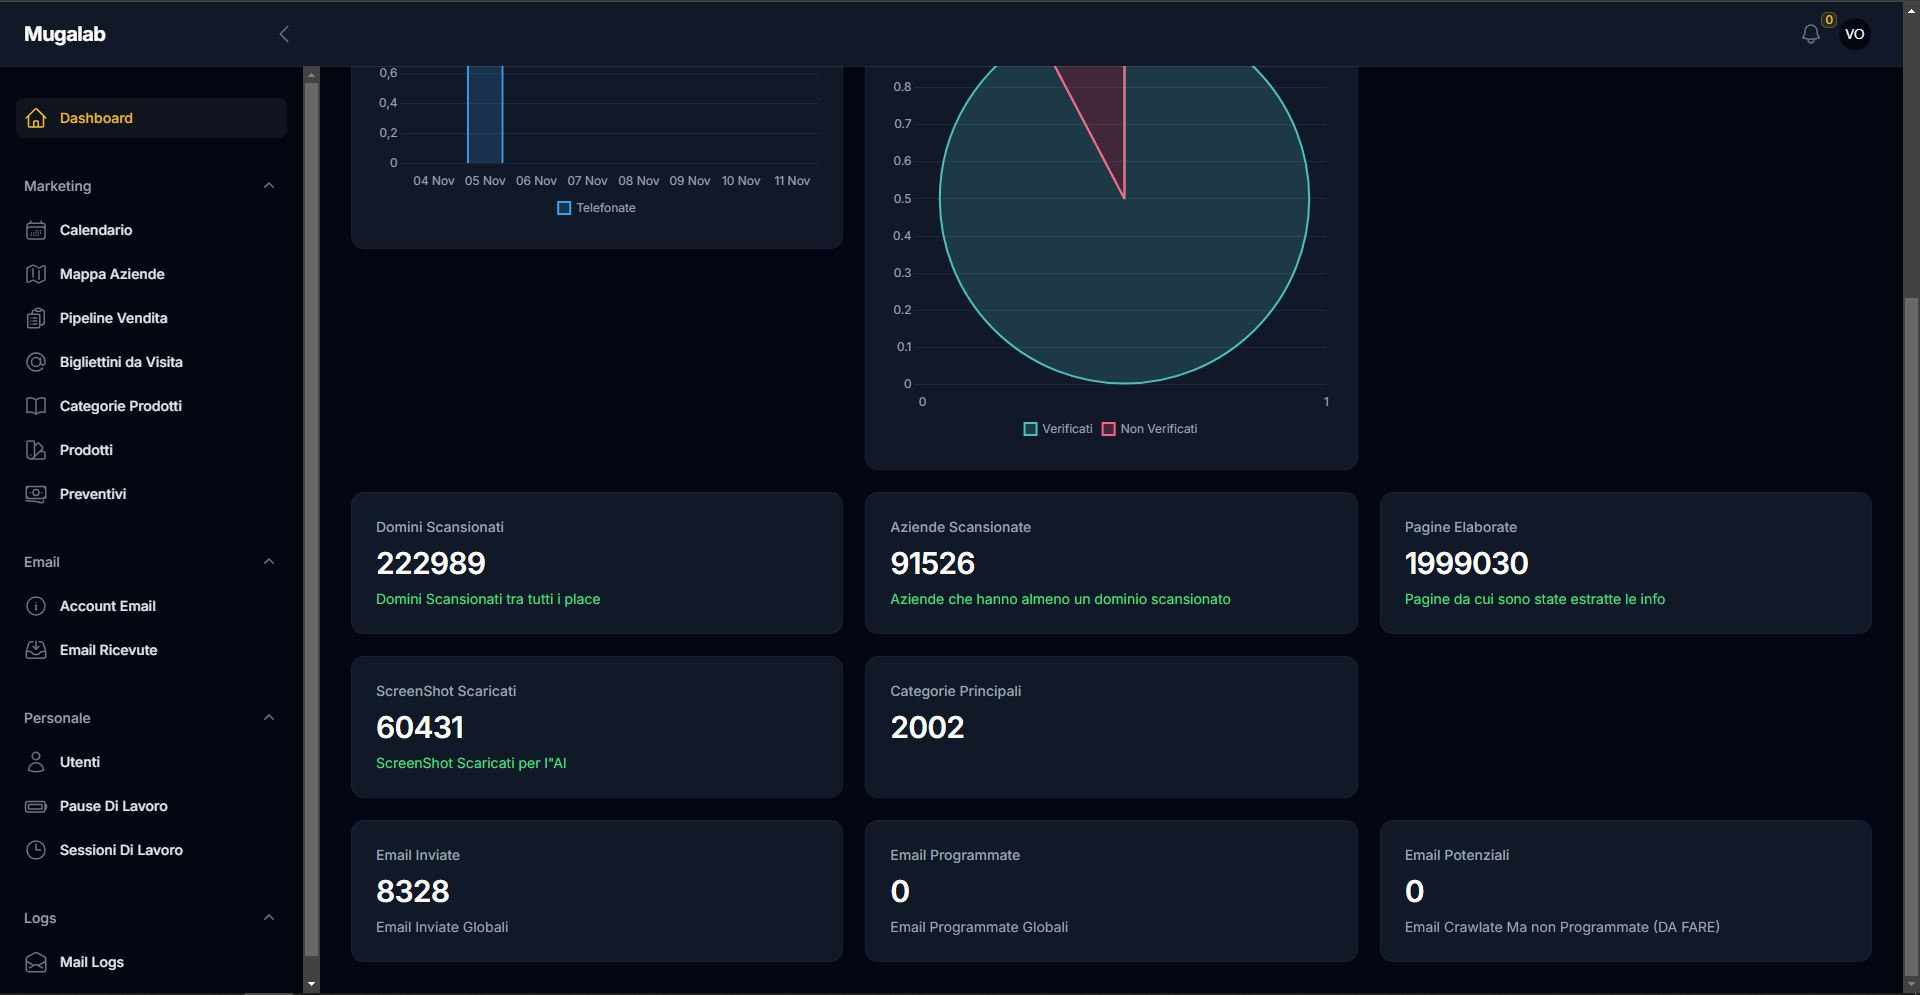
\includegraphics[width=0.8\columnwidth]{progetto/Home_page.png} 
        \caption{Home page di SalesCRM}
        \label{fig:salesCRM-home}
      \end{figure}

    \item Il modulo contenente il calendario (Fig.~\ref{fig:salesCRM-calendario}) è utile per pianificare appuntamenti e visite.
    
    \begin{figure}[!h] 
        \centering 
        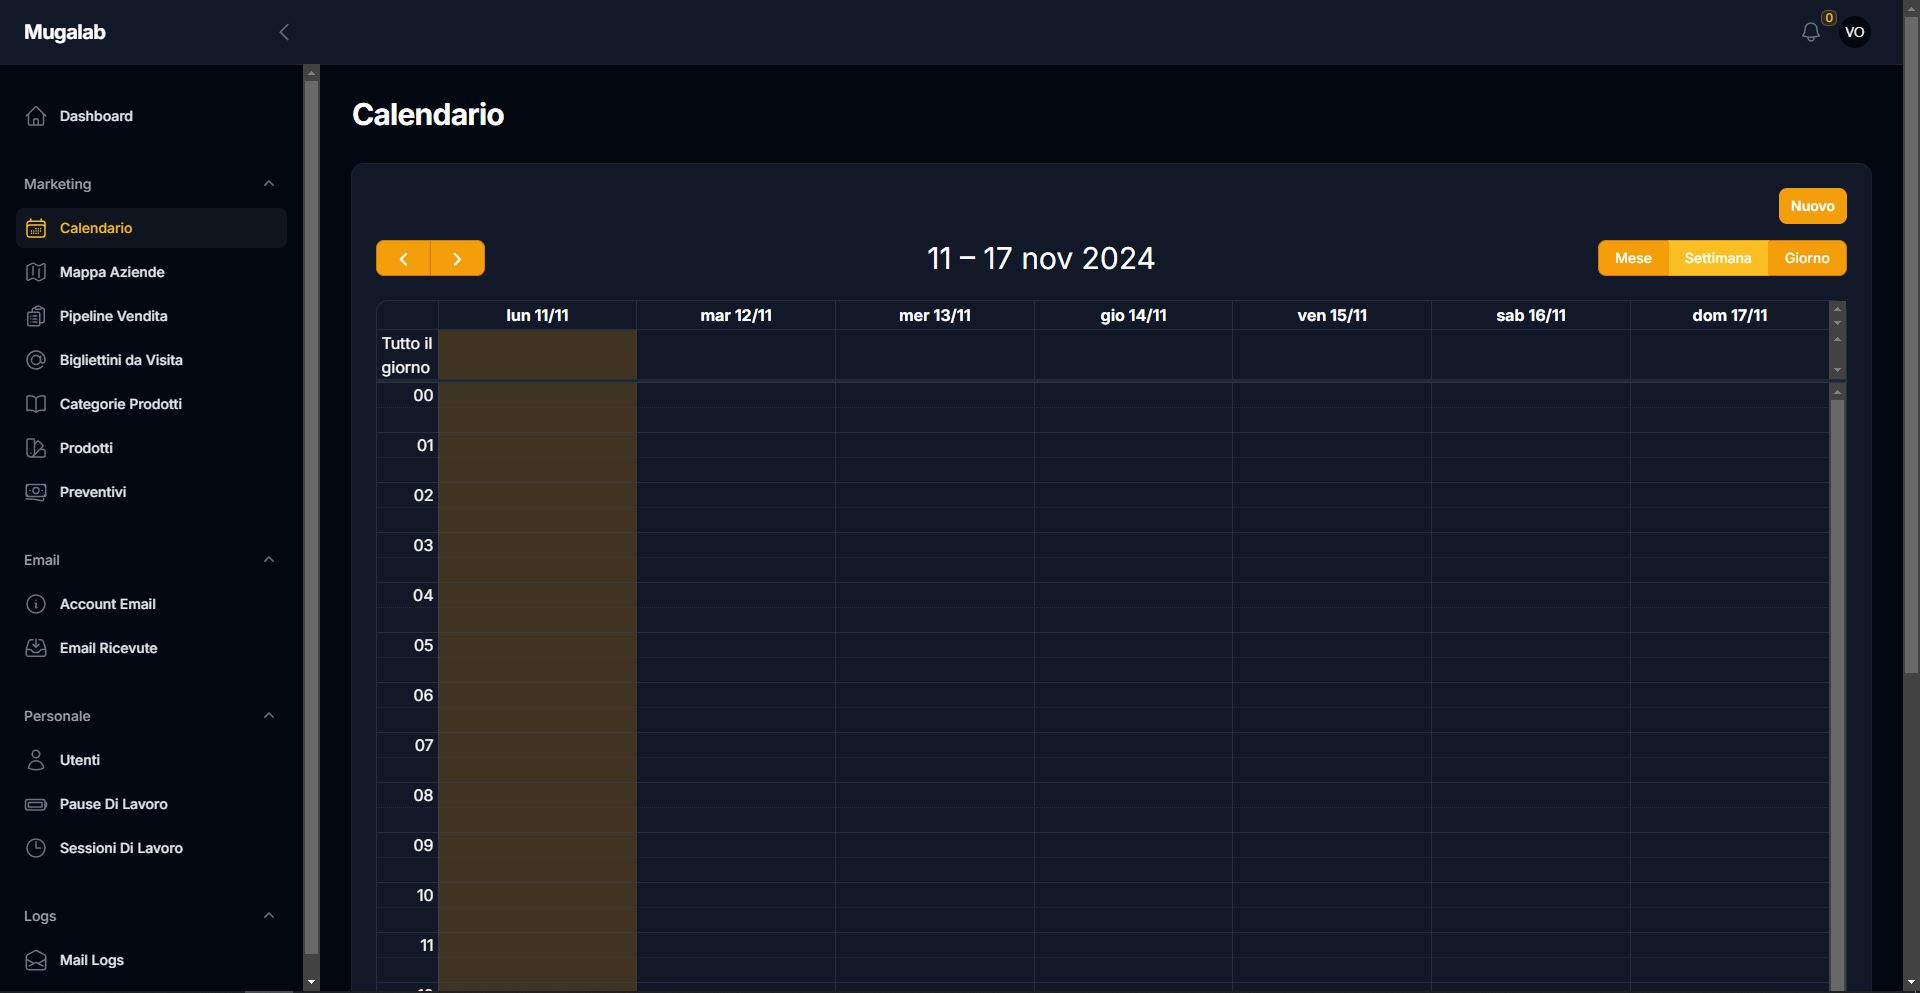
\includegraphics[width=0.8\columnwidth]{progetto/Calendario.png} 
        \caption{Calendario contenuto all'interno di SalesCRM}
        \label{fig:salesCRM-calendario}
      \end{figure}

    \item La sezione della mappa (Fig.~\ref{fig:salesCRM-mappa}) viene sfruttato per conoscere il posizionamento dei clienti e organizzare incontri locali.
    
    \begin{figure}[!h] 
        \centering 
        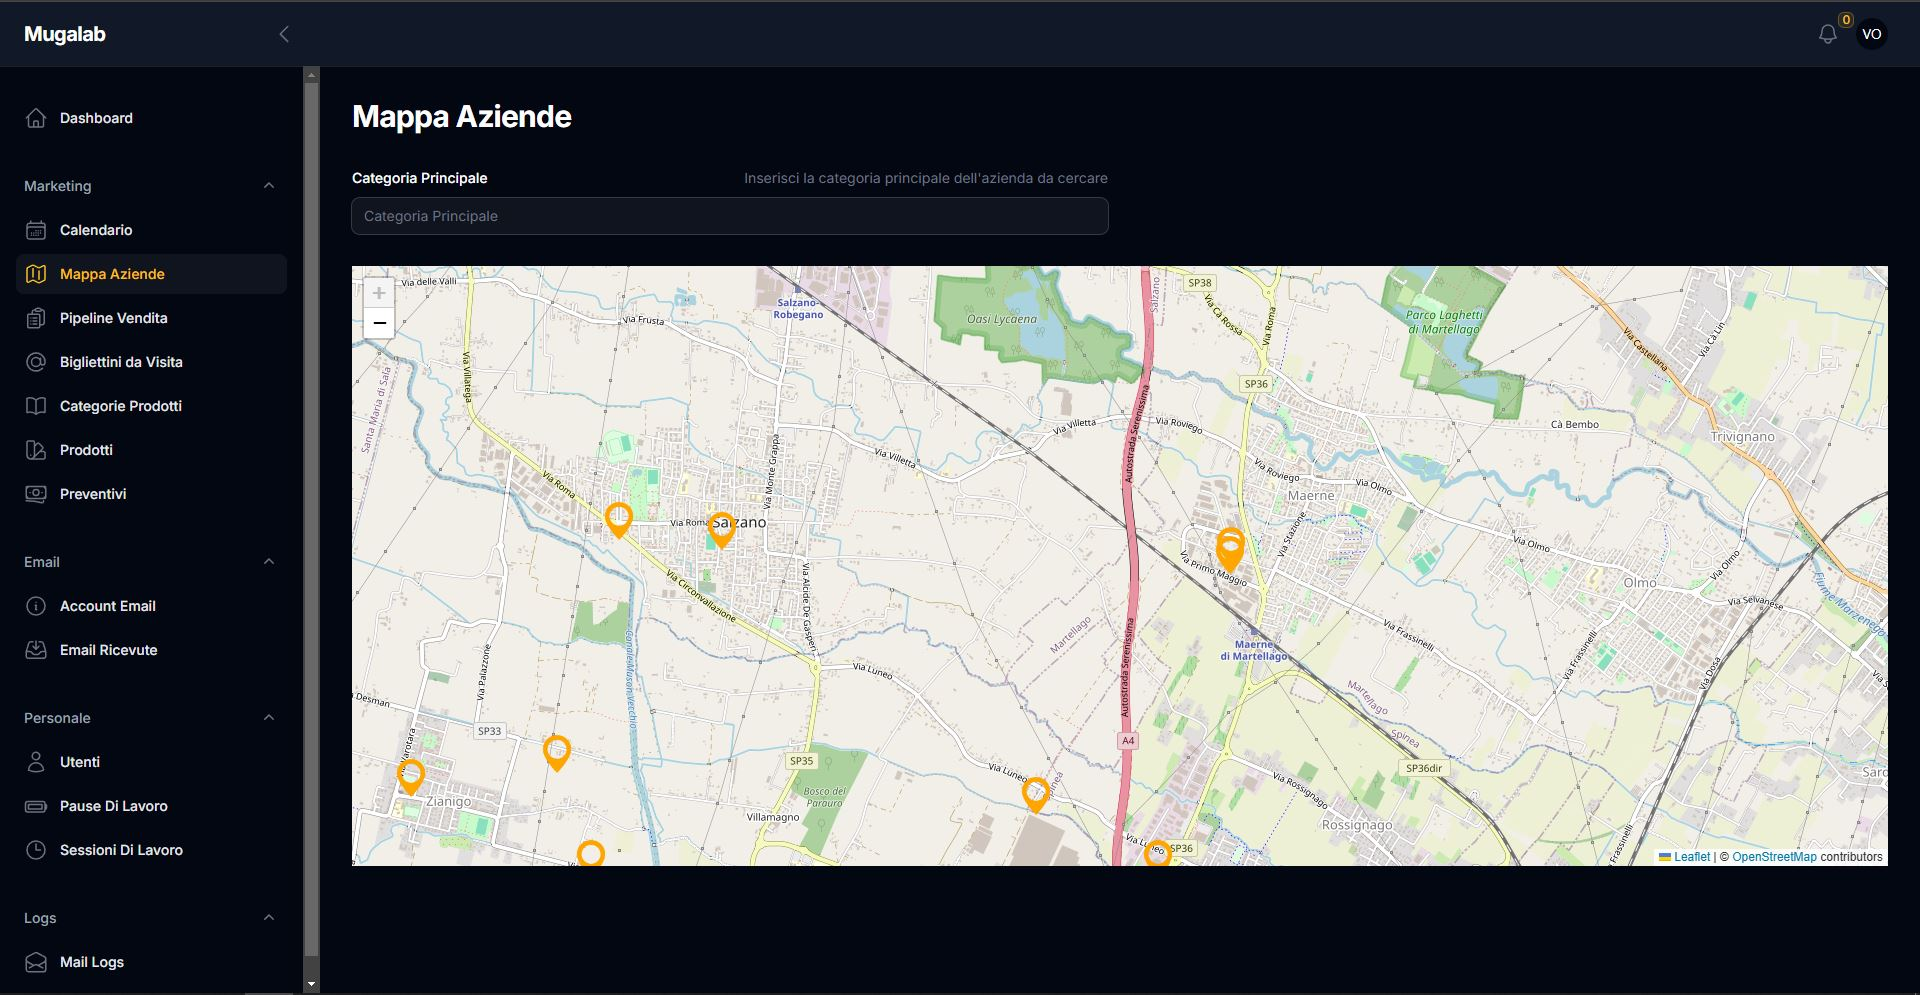
\includegraphics[width=0.8\columnwidth]{progetto/Mappa.png} 
        \caption{Mappa contenuta all'interno di SalesCRM}
        \label{fig:salesCRM-mappa}
      \end{figure}
    
\end{itemize}

\newpage

\subsection{Integrazione}
\begin{itemize}
    \item Raccolta di dati: l'applicativo ha una funzionalità di web-scraping che raccoglie i link dei siti web di tutti i potenziali clienti, il compito del tirocinante è quello di creare un workflow automatico che si integri con il web-scraper per acquisire screenshot delle varie pagine del sito web. 
    \item Clusterizzazione: la fase successiva alla raccolta dei dati consiste nello sviluppo di una IA addestrata in maniera non supervisionata che sia in grado di suddividere le varie immagini in clusters, differenziati in base alle caratteristiche riconosciute in ogni sito. 
    \item IA classificativa: in seguito alla raccolta di un dataset di dimensioni congrue si procede alla suddivisione manuale degli screenshot precedentemente clusterizzati su una base qualitativa (siti migliorabili e siti ottimi); questo processo viene svolto con l'ottica dell'addestramento di una IA classificativa.
    L'IA addestrata in maniera supervisionata ha l'obiettivo di affidare un punteggio in valori centesimali a ogni sito. 
    \item Invio di e-mail automatizzato: l'automazione della posta elettronica procede con l'invio di e-mail personalizzate ai proprietari dei siti web che hanno ricevuto una valutazione scarsa, per offrire loro un servizio di miglioramento.
\end{itemize}

\section{Analisi e gestione dei rischi}
Durante l'analisi del progetto lo stagista ha individuato alcuni rischi in cui potrà incorrere.
Nella lista seguente sono elencati i rischi e le soluzioni ideate.\\

\begin{risk}{Rimodulazione dell'attività}
    \riskdescription{dopo un mese dall’inizio dello stage lo studente è stato riposizionato sul progetto attuale scartando il progetto precedente e trovandosi dunque con meno settimane a disposizione per la produzione}
    \risksolution{ridimensionamento delle attività e richieste di supporto più frequenti}
    \label{risk: tempistiche ristrette} 
\end{risk}

\begin{risk}{Approccio sperimentale}
    \riskdescription{il progetto prevede dei contributi originali e sperimentali per cui non sono disponibili soluzioni già pronte}
    \risksolution{auto apprendimento tramite tutorial on-line e richiesta di coinvolgimento di colleghi più esperti nell'ambito}
    \label{risk:conoscenze scarse} 
\end{risk}

\begin{risk}{Costo dell'Addestramento}
    \riskdescription{l'addestramento dell'intelligenza artificiale richiede l'utilizzo di potenti GPU di cui spesso l'hardware a disposizione è sprovvisto}
    \risksolution{utilizzo del server aziendale per l’addestramento su CPU, ottenendo un compromesso tra costi e tempo di addestramento}
    \label{risk:hardware} 
\end{risk}

\begin{risk}{Quantità di dati di training insufficiente}
    \riskdescription{l'IA necessita una grande quantità di dati in input per effettuare un training efficace}
    \risksolution{aumento manuale del dataset e ricerca di dataset già pronti on-line}
    \label{risk:hardware} 
\end{risk}

%AGGIUNGERE ALTRI RISCHI

\newpage

\begin{risk}{Risultati della clusterizzazione non soddisfacenti}
    \riskdescription{il clustering potrebbe risultare non conforme alle aspettative}
    \risksolution{valutare la quantità di cluster da creare e sperimentare con altri metodi di clustering}
    \label{risk:hardware} 
\end{risk}


\begin{risk}{Overfitting del modello}
    \riskdescription{il modello IA fornisce valutazioni accurate solo per le immagini utilizzate durante il training}
    \risksolution{sperimentare con metodi per la risoluzione dell'overfit (dropout, cross-validation, ecc...)}
    \label{risk:hardware} 
\end{risk}

\section{Obiettivi}
Gli obiettivi hanno lo scopo di delineare il percorso che lo studente deve affrontare per portare a termine il progetto nella maniera desiderata dall'azienda.
Sono suddivisibili in:
\begin{itemize}
    \item \textbf{O}: obbligatori
    \item \textbf{D}: desiderabili
    \item \textbf{F}: facoltativi
\end{itemize}

\begin{table}[h!]
    \centering
    \begin{tabularx}{0.8\textwidth}{|c|X|}
    \hline
    \textbf{Codice} & \textbf{Descrizione} \\
    \hline
    O01 & Implementare un sistema robusto per la cattura degli screenshot, assicurando l’integrazione con il
        database per l’archiviazione e l’analisi. \\
    \hline
    O02 & Garantire la creazione di una documentazione tecnica completa che supporti sia l’uso che la manutenzione  del sistema sviluppato. \\
    \hline
    O03 & Creazione di un IA in grado di suddividere in cluster i siti web. \\
    \hline
    O04 & Creazione di un IA classificativa in grado di assegnare un punteggio ai siti-web analizzati.\\
    \hline
    D01 & Aggiungere la valutazione creata dall'IA nel database utilizzato dal CRM.\\
    \hline
    D02 & Automatizzare l'invio di e-mail alle aziende che hanno ottenuto una valutazione scarsa.\\
    \hline
    F01 & Migliorare la raccolta dei dati delle aziende dal web\\
    \hline
    F02 & Aggiornare automaticamente la valutazione dei siti web\\
    \hline
    \end{tabularx}
    \caption{Tabella degli obiettivi}
    \end{table}

\section{Pianificazione}

    \chapter{Analisi dei requisiti}
\label{cap:analisi-requisiti}

\intro{Breve introduzione al capitolo}\\

\section{Casi d'uso}

Per lo studio dei casi di utilizzo del prodotto sono stati creati dei diagrammi.
I diagrammi dei casi d'uso (in inglese \emph{Use Case Diagram}) sono diagrammi di tipo \gls{uml} dedicati alla descrizione delle funzioni o servizi offerti da un sistema, così come sono percepiti e utilizzati dagli attori che interagiscono col sistema stesso.
Essendo il progetto finalizzato alla creazione di un tool per l'automazione di un processo, le interazioni da parte dell'utilizzatore devono essere ovviamente ridotte allo stretto necessario. Per questo motivo i diagrammi d'uso risultano semplici e in numero ridotto.

\begin{figure}[!h] 
    \centering 
    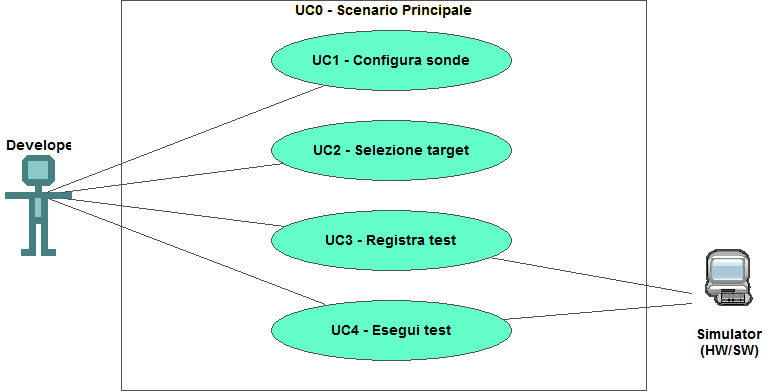
\includegraphics[width=0.9\columnwidth]{usecase/scenario-principale} 
    \caption{Use Case - UC0: Scenario principale}
\end{figure}

\begin{usecase}{0}{Scenario principale}
\usecaseactors{Sviluppatore applicativi}
\usecasepre{Lo sviluppatore è entrato nel plug-in di simulazione all'interno dell'IDE}
\usecasedesc{La finestra di simulazione mette a disposizione i comandi per configurare, registrare o eseguire un test}
\usecasepost{Il sistema è pronto per permettere una nuova interazione}
\label{uc:scenario-principale}
\end{usecase}

\section{Tracciamento dei requisiti}

Da un'attenta analisi dei requisiti e degli use case effettuata sul progetto è stata stilata la tabella che traccia i requisiti in rapporto agli use case.\\
Sono stati individuati diversi tipi di requisiti e si è quindi fatto utilizzo di un codice identificativo per distinguerli.\\
Il codice dei requisiti è così strutturato R(F/Q/V)(N/D/O) dove:
\begin{enumerate}
	\item[R =] requisito
    \item[F =] funzionale
    \item[Q =] qualitativo
    \item[V =] di vincolo
    \item[N =] obbligatorio (necessario)
    \item[D =] desiderabile
    \item[Z =] opzionale
\end{enumerate}
Nelle tabelle \ref{tab:requisiti-funzionali}, \ref{tab:requisiti-qualitativi} e \ref{tab:requisiti-vincolo} sono riassunti i requisiti e il loro tracciamento con gli use case delineati in fase di analisi.

\newpage

\begin{table}%
\caption{Tabella del tracciamento dei requisti funzionali}
\label{tab:requisiti-funzionali}
\begin{tabularx}{\textwidth}{lXl}
\hline\hline
\textbf{Requisito} & \textbf{Descrizione} & \textbf{Use Case}\\
\hline
RFN-1     & L'interfaccia permette di configurare il tipo di sonde del test & UC1 \\
\hline
\end{tabularx}
\end{table}%

\begin{table}%
\caption{Tabella del tracciamento dei requisiti qualitativi}
\label{tab:requisiti-qualitativi}
\begin{tabularx}{\textwidth}{lXl}
\hline\hline
\textbf{Requisito} & \textbf{Descrizione} & \textbf{Use Case}\\
\hline
RQD-1    & Le prestazioni del simulatore hardware deve garantire la giusta esecuzione dei test e non la generazione di falsi negativi & - \\
\hline
\end{tabularx}
\end{table}%

\begin{table}%
\caption{Tabella del tracciamento dei requisiti di vincolo}
\label{tab:requisiti-vincolo}
\begin{tabularx}{\textwidth}{lXl}
\hline\hline
\textbf{Requisito} & \textbf{Descrizione} & \textbf{Use Case}\\
\hline
RVO-1    & La libreria per l'esecuzione dei test automatici deve essere riutilizzabile & - \\
\hline
\end{tabularx}
\end{table}%

    \chapter{Progettazione e codifica}
\label{cap:progettazione-codifica}

\intro{Breve introduzione al capitolo}\\

\section{Tecnologie e strumenti}
\label{sec:tecnologie-strumenti}

Di seguito viene data una panoramica delle tecnologie e strumenti utilizzati.

\subsection*{Tecnologia 1}
Descrizione Tecnologia 1.

\subsection*{Tecnologia 2}
Descrizione Tecnologia 2

\section{Ciclo di vita del software}
\label{sec:ciclo-vita-software}

\section{Progettazione}
\label{sec:progettazione}

\subsubsection{Namespace 1} %**************************
Descrizione namespace 1.

\begin{namespacedesc}
    \classdesc{Classe 1}{Descrizione classe 1}
    \classdesc{Classe 2}{Descrizione classe 2}
\end{namespacedesc}


\section{Design Pattern utilizzati}

\section{Codifica}

    \chapter{Progettazione e codifica}
\label{cap:progettazione-codifica}

    \chapter{Conclusioni}
\label{cap:conclusioni}

\section{Consuntivo finale}

\section{Raggiungimento degli obiettivi}

\section{Conoscenze acquisite}

\section{Valutazione personale}


    \appendix
    \chapter{Appendice A}

\epigraph{Citazione}{Autore della citazione}


    \backmatter
    \printglossary[type=\acronymtype, title=Acronimi e abbreviazioni, toctitle=Acronimi e abbreviazioni]
    \printglossary[type=main, title=Glossario, toctitle=Glossario]

    \cleardoublepage
\chapter{Bibliografia}

\nocite{*}

% Print book bibliography
\printbibliography[heading=subbibliography,title={Riferimenti bibliografici},type=book]

% Print site bibliography
\printbibliography[heading=subbibliography,title={Siti web consultati},type=online]

\end{document}
